\documentclass{article}
\usepackage{fancyhdr}
\usepackage{extramarks}
\usepackage{amsmath}
\usepackage{amsthm}
\usepackage{amsfonts}
\usepackage{tikz}
\usepackage[plain]{algorithm}
\usepackage{algpseudocode}
\usepackage{listings}
\usepackage{amssymb}
\usetikzlibrary{automata,positioning,graphs}

\usepackage{color}

\definecolor{dkgreen}{rgb}{0,0.6,0}
\definecolor{gray}{rgb}{0.5,0.5,0.5}
\definecolor{mauve}{rgb}{0.58,0,0.82}

\lstset{frame=tb,
  language=Python,
  aboveskip=3mm,
  belowskip=3mm,
  showstringspaces=false,
  columns=flexible,
  basicstyle={\small\ttfamily},
  numbers=none,
  numberstyle=\tiny\color{gray},
  keywordstyle=\color{blue},
  commentstyle=\color{dkgreen},
  stringstyle=\color{mauve},
  breaklines=true,
  breakatwhitespace=true,
  tabsize=3
}
%
% Basic Document Settings
%

\topmargin=-0.45in
\evensidemargin=0in
\oddsidemargin=0in
\textwidth=6.5in
\textheight=9.0in
\headsep=0.25in

\linespread{1.1}

\pagestyle{fancy}
\lhead{\hmwkAuthorName}
\chead{\hmwkClass\: \hmwkTitle}
\rhead{\firstxmark}
\lfoot{\lastxmark}
\cfoot{\thepage}

\renewcommand\headrulewidth{0.4pt}
\renewcommand\footrulewidth{0.4pt}

\setlength\parindent{0pt}


% Create Problem Sections
%

\newcommand{\enterProblemHeader}[1]{
    \nobreak\extramarks{}{Problem \arabic{#1} continued on next page\ldots}\nobreak{}
    \nobreak\extramarks{Problem \arabic{#1} (continued)}{Problem \arabic{#1} continued on next page\ldots}\nobreak{}
}

\newcommand{\exitProblemHeader}[1]{
    \nobreak\extramarks{Problem \arabic{#1} (continued)}{Problem \arabic{#1} continued on next page\ldots}\nobreak{}
    \stepcounter{#1}
    \nobreak\extramarks{Problem \arabic{#1}}{}\nobreak{}
}

\setcounter{secnumdepth}{0}
\newcounter{partCounter}
\newcounter{homeworkProblemCounter}
\setcounter{homeworkProblemCounter}{1}
\nobreak\extramarks{Problem \arabic{homeworkProblemCounter}}{}\nobreak{}

%
% Homework Problem Environment
%
% This environment takes an optional argument. When given, it will adjust the
% problem counter. This is useful for when the problems given for your
% assignment aren't sequential. See the last 3 problems of this template for an
% example.
%
\newenvironment{homeworkProblem}[1][-1]{
    \ifnum#1>0
        \setcounter{homeworkProblemCounter}{#1}
    \fi
    \section{Problem \arabic{homeworkProblemCounter}}
    \setcounter{partCounter}{1}
    \enterProblemHeader{homeworkProblemCounter}
}{
    \exitProblemHeader{homeworkProblemCounter}
}

%
% Homework Details
%   - Title
%   - Due date
%   - Class
%   - Section/Time
%   - Instructor
%   - Author
%
\newcommand{\hmwkNum}{8}
\newcommand{\hmwkTitle}{Homework\ \#\hmwkNum}
\newcommand{\hmwkDueDate}{November 25, 2019}
\newcommand{\hmwkClass}{CSCI971 Advance Computer Security}
\newcommand{\hmwkClassInstructor}{Chen Jiageng}
\newcommand{\hmwkAuthorName}{\textbf{Mei Wangzhihui}}
\newcommand{\hmwkAuthorNum}{\textbf{2019124044}}
%
% Title Page
%

\title{
    \vspace{2in}
    \textmd{\textbf{\hmwkClass:\\ \hmwkTitle}}\\
    % \normalsize\vspace{0.1in}\small{Due\ on\ \hmwkDueDate\ at 3:10pm}\\
    % \vspace{0.1in}\large{\textit{\hmwkClassInstructor\ \hmwkClassTime}}
    \vspace{3in}
}

\author{\hmwkAuthorName\ \\ \hmwkAuthorNum}
\date{}

\renewcommand{\part}[1]{\textbf{\large Part \Alph{partCounter}}\stepcounter{partCounter}\\}

%
% Various Helper Commands
%

% Useful for algorithms
\newcommand{\alg}[1]{\textsc{\bfseries \footnotesize #1}}

% For derivatives
\newcommand{\deriv}[1]{\frac{\mathrm{d}}{\mathrm{d}x} (#1)}

% For partial derivatives
\newcommand{\pderiv}[2]{\frac{\partial}{\partial #1} (#2)}

% Integral dx
\newcommand{\dx}{\mathrm{d}x}

% Alias for the Solution section header
\newcommand{\solution}{\textbf{\large Solution}}

% Probability commands: Expectation, Variance, Covariance, Bias
\newcommand{\E}{\mathrm{E}}
\newcommand{\Var}{\mathrm{Var}}
\newcommand{\Cov}{\mathrm{Cov}}
\newcommand{\Bias}{\mathrm{Bias}}

\begin{document}

\maketitle

\clearpage

\begin{homeworkProblem}
For a RSA trapdoor function, if it is used directly as the encryption, then We assume the Challenger $\mathcal{C}$ produce RSA params with $G()$ and get $pk=(N,e),sk=(N,d)$, then Adversary produce two message $m_1,m_2$ and $|m_1|=|m_2|$, Challenger select $b$ randomly and perform encryption $c_b=E(pk,m_b)=m_b^e$, the decryption should be $m_b=c_b^d$. The Adversary get $pk$ and generate $b$. 
\begin{figure}[h]
    \centering %图片居中
    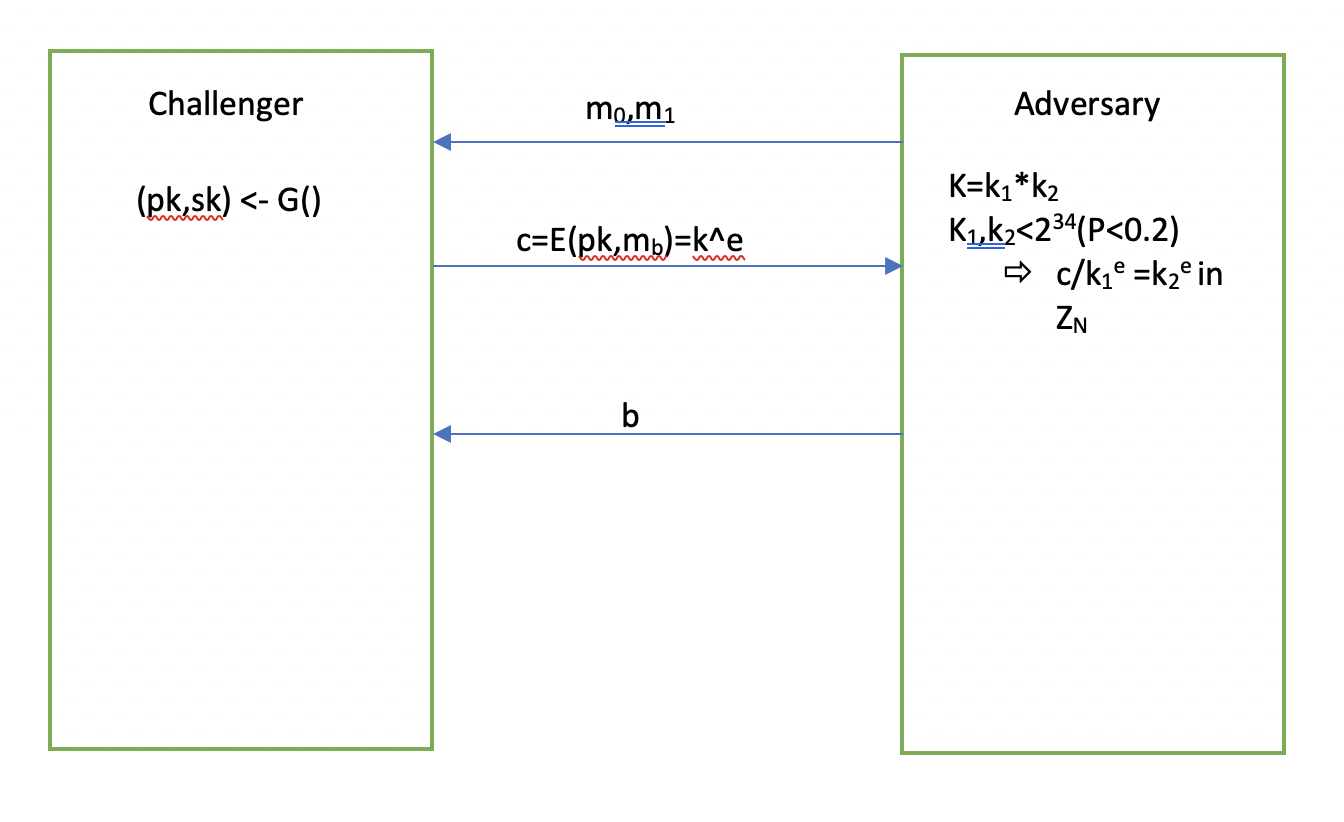
\includegraphics[width=1.0\textwidth]{attackgamersa} %插入图片,[]中设置图片大小,{}中是图片文件名
    \caption{Attack Game} %最终文档中希望显示的图片标题
\end{figure}

We suppose k is 64bits, $k\in\{0,...2^{64}\}$, it get $c=k^e$ in $Z_N$ if $k=k_1*k_2$ where $k_1,k_2<2^34$ ($Pr\approx0.2$) then $c/k_1^e=k_2^e$ in $Z_N$, firstly, Adversary $\mathcal{A}$ can build table of $k_2^e=c/1^e,c/2^e...,c/2^{34e}$ then he can itertablely test if $k_2^e$ is in table. 
he can output matching $k_1,k_2$.
\end{homeworkProblem}

\clearpage
\begin{homeworkProblem}
    
    \begin{figure}[h]
        \centering %图片居中
        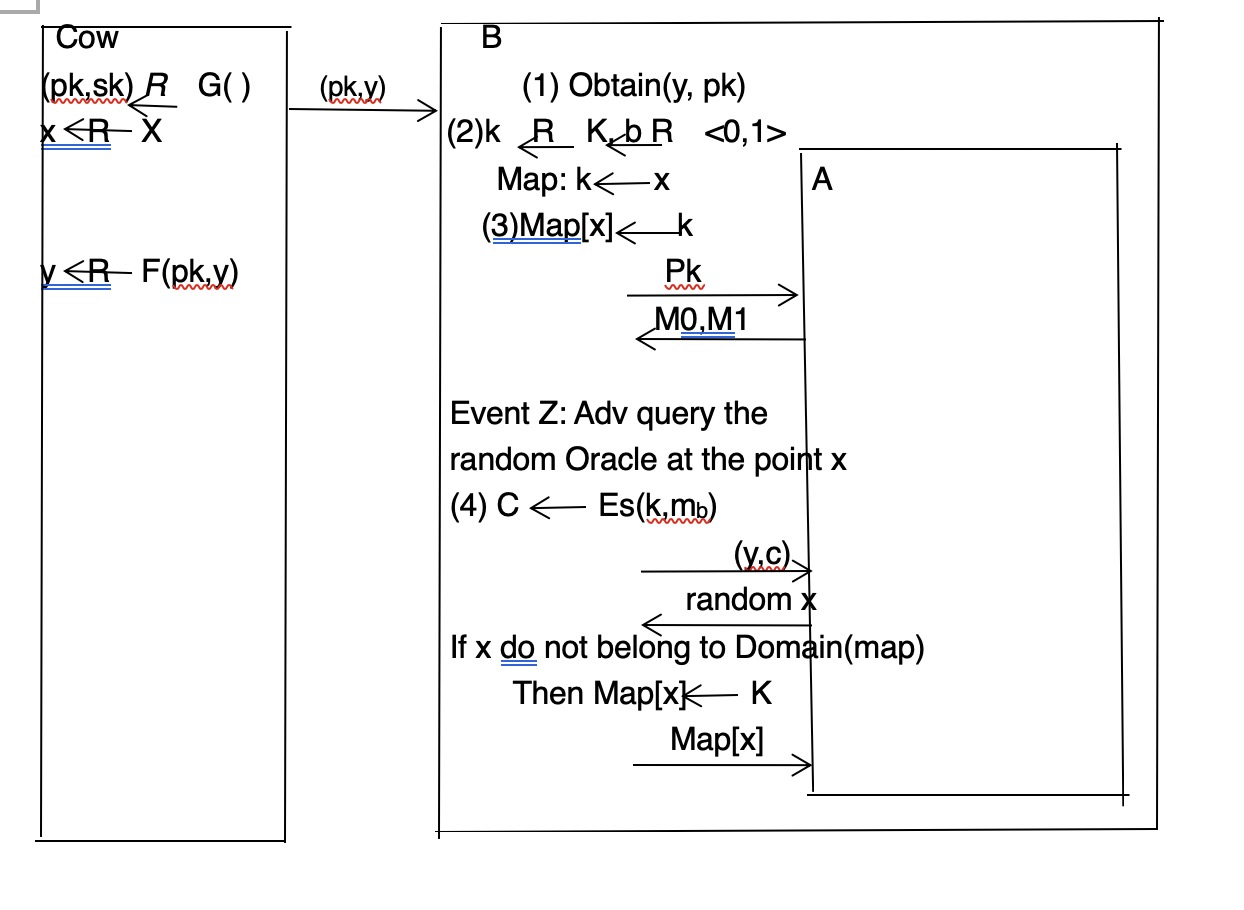
\includegraphics[width=1.0\textwidth]{a8t2} %插入图片,[]中设置图片大小,{}中是图片文件名
        \caption{} %最终文档中希望显示的图片标题
    \end{figure}
    As $SSadv$[A,$\epsilon_{TDF}$] = 2$SS^{ro}adv^{*}[A,\epsilon_{TDF}]$. 
    We need to prove:
    $$
        SS^{*}{adv}[A,\epsilon_{TDF}] \leq OWadv[B_{ow},T] + SSadv^{*}[B_{s},\epsilon_{s}]
    $$
    

    

    We can defind Game0 and Game1 like this:
    Set $W_{j}$ as $\widehat{b}$ = b in Game j, (j=0,1). 
    
    Then get $|Pr[W_1]|-|Pr[W_0]|$ is negligible and $|Pr[W1]|\approx1/2$.
    
    Then $SS^{ro}adv^{*}[A,\epsilon_{TDF}]$ = |Pr[W0]-1/2| is negligible.

    Game0: Adversary can make any number of random oracle queries but at most one encryption query. 

    Game1: The (PK,y) is obtained by Cow .\\

    
    Set Z: Adversary queries the random oracle at the point x in Game1. At this time, Game0 and Game1 proceed identically unless Z occurs, So We can have:\\
    \centerline{$|Pr[W1]-Pr[W0]| <= Pr[Z]$}
    If event Z happens, then one of the adv's random queries is the inverse of y under $F(pk,)$. In Game1, the value of x is only used to define y. 
    
    Then use  that breaks the OW for TDF with advantage equal to Pr[Z].\\
    Lets view Game1 and the game between Bow and Cow. By the definition above Z occurs if and only if x $\in$ Domain(Map) when Bow finishes its game. So we can indicate:\\
    \centerline{$Pr[Z]=OWadv[B_{ow},T]$}
    Observe that in Game1,the key k is only used to encrypt the challenge plaintext. As such, the adversary is attacking the bit-guessing version as Attack Game 2.1 from which we can know that:\\
    \centerline{$|Pr[W-{1}]-1/2| = SSadv^{*}[B_{s}],\epsilon_{s}$}
    Then delete the process of (2),(3) change (4) to forward$(m_{0},m_{1})$ to Cs, obtaining c. Additionly"\\
     When A outputs $\widehat{b}$.then output $\widehat{b}$\\
    Then we can conclude\\
     \centerline{$SS^{ro}$adv[A,$\epsilon_{TDF}]$ <= 2$OWadv[B_{ow},T]$ + $SSadv[B_{s},E_{s}]$ }
    

\end{homeworkProblem}

\end{document}